\chapter{Evaluation}
\label{ch:Evaluation}

\abstract{This chapter provides the analysis of the statistics gathered from the final implementations. As stated in the introduction the evaluation considers raw performance characteristics as well as developer productivity from the previous chapter.
}

Preface: All data in this chapter was gathered from a high performance computer by courtesy of the \gls{dkrz}. The machine has access to 48 singlecore processors and xxx GB of memory. It is therefore ideal to compare shared memory performance on a large scale.

\section{Performance}
\label{sec:Evaluaton::Performance}

\begin{table}[htb]
    \centering
    \begin{tabular}{rccc}
        \toprule
        % Header
            threads/goroutines
            & C
            & Go
            & Rust \\
        \midrule

            1
            & xx:xx:xx
            & 16:48:19
            & 14:15:06 \\

            2
            & xx:xx:xx
            & 10:21:36
            & xx:xx:xx \\

            4
            & xx:xx:xx
            & 05:58:35
            & xx:xx:xx \\

            8
            & xx:xx:xx
            & 03:01:54
            & xx:xx:xx \\

            12
            & xx:xx:xx
            & 02:06:08
            & xx:xx:xx \\

            24
            & xx:xx:xx
            & 01:13:47
            & xx:xx:xx \\

            48
            & xx:xx:xx
            & 00:53:54
            & xx:xx:xx \\

        \bottomrule
    \end{tabular}
    \caption{Execution time of the final applications (100.000 nodes)}
    \label{tb:final_execution_time}
\end{table}

\begin{table}[htb]
    \centering
    \begin{tabular}{rccc}
        \toprule
        % Header
            threads/goroutines
            & C
            & Go
            & Rust \\
        \midrule

            1
            & 1.0000
            & 1.0000
            & 1.0000 \\

            2
            & xx:xx:xx
            & 1.6221
            & xx:xx:xx \\

            4
            & xx:xx:xx
            & 2.8119
            & xx:xx:xx \\

            8
            & xx:xx:xx
            & 5.5432
            & xx:xx:xx \\

            12
            & xx:xx:xx
            & 7.9941
            & xx:xx:xx \\

            24
            & xx:xx:xx
            & 13.6659
            & xx:xx:xx \\

            48
            & xx:xx:xx
            & 18.7072
            & xx:xx:xx \\

        \bottomrule
    \end{tabular}
    \caption{Parallel speedup of the final applications (100.000 nodes)}
    \label{tb:final_speedup}
\end{table}

\section{Additional metrics / productivity}
\label{sec:Evaluation::Metrics}

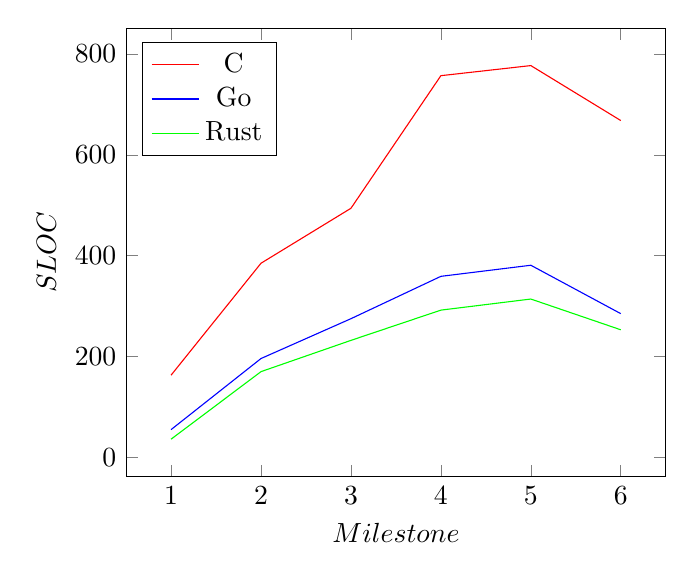
\begin{tikzpicture}
    \begin{axis}[
        xlabel=$Milestone$,
        ylabel=$SLOC$,
        xtick={1,2,3,4,5,6},
        legend pos=north west
    ]

    \addplot[red] plot coordinates {
        (1,163)
        (2,385)
        (3,494)
        (4,757)
        (5,777)
        (6,668)};
    \addlegendentry{C}

    \addplot[color=blue] plot coordinates {
        (1,55)
        (2,196)
        (3,275)
        (4,359)
        (5,381)
        (6,285)};
    \addlegendentry{Go}

    \addplot[color=green] plot coordinates {
        (1,36)
        (2,170)
        (3,232)
        (4,292)
        (5,314)
        (6,253)};
    \addlegendentry{Rust}
    \end{axis}
\end{tikzpicture}
